\documentclass{beamer}
\usepackage[utf8]{inputenc}
\usepackage{amsmath}
\usepackage{amsfonts}
\usepackage{amssymb}
\usepackage{multicol}
\usepackage{graphics}
\usetheme{CambridgeUS}
\newcommand{\ds}{\displaystyle}
\pagestyle{empty}
\title{Verificaci{\'o}n de la existencia de un ciclo hamiltoniano en un grafo aleatorio}
\date{}
\begin{document}
\begin{frame}
\begin{center}
\textbf{Unidad Acad{\'e}mica}: 
\\Facultad de Ciencias\\
\textbf{Curso y secci{\'o}n}: 
\\Introducci{\'o}n a la Estad{\'i}stica y Probabilidades(CM-274 "A")\\
\textbf{Semestre}: 
\\2018-II\\
\textbf{Profesores}:
\\ Zamudio Fernando - C{\'e}sar Lara\\
\textbf{Integrantes}:\\
/Jaafar Farut Sahua Torres/\\
/Franklin F{\'e}lix Rivera Granados/\\
/Briguitte Stefany Maquera de la Cruz/
\end{center}
\end{frame}
\begin{frame}
\titlepage
\end{frame}
\begin{frame}
\frametitle{Introducci{\'o}n}
\underline{Definiciones}:\\
* \textbf{Grafo}: Es un diagrama que representa mediante vertices y aristas las relaciones entre pares de elementos y que se usa para resolver problemas l{\'o}gicos, topol{\'o}gicos y de c{\'a}lculo combinatorio.\\
* \textbf{Grafo hamiltoniano}: Es aquel grafo que tiene un ciclo hamiltoniano el cual recorre una sola vez cada vertice y el vertice final sea adyacente al primero, de esa forma contiene un camino hamiltoniano.\\
¿\underline{C{\'o}mo identificar un grafo hamiltoniano}?\\
Contrario al caso de los grafos eulerianos, para el caso de los grafos hamiltonianos no se conoce ninguna condici{\'o}n necesaria y suficiente que los caracterice. Esto es lamentable porque en muchas aplicaciones es fundamental poder determinar si un grafo es hamiltoniano.\\
\end{frame}
\begin{frame}
\begin{center}
Ejemplos de Grafos hamiltonianos
\end{center}
\begin{minipage}{4cm}
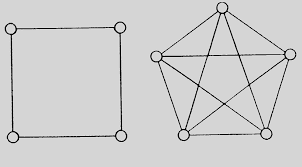
\includegraphics[scale=0.58]{grafo.PNG}
\end{minipage}
\begin{center}
\textbf{\underline{Objetivo del Proyecto}}
\end{center}
* Es la verificaci{\'o}n de un grafo y determinar si es o no es hamiltoniano  pues ya que aunque no hay condici{\'o}n o formula totalmente eficiente para su demostracion, podemos aproximarnos utilizando ciertas condiciones.\\
* El implemento de la programacion mediante el uso del Lenguaje R en nuestro proyecto para dicha verificacion\\
* El uso de algunas formulas y teoremas estadisticos para la determinaci{\'o}n de un grafo y verificar si es o no es hamiltoniano 
\end{frame}
\begin{frame}
\tableofcontents
\end{frame}
\section{Estado del arte}
\begin{frame}
\frametitle{Estado del arte}
* \textbf{Libro(PDF):} Matem{\'a}tica Discreta "Teoria de Grafos"\\
\textbf{autores:} Merce Claverol, Ester Simo y Marisa Zaragoza\\
\textbf{Tema 2:} p{\'a}ginas(38-39)\\
* \textbf{Libro(PDF):} Teorema de Dirac y Ore (aplicaciones de la matetica discreta en la vide real)\\
\textbf{autores:} Alberto Conejero y Cristian J{\'o}rdan\\
* \textbf{Video(Tutorial):} Introducci{\'o}n a los Grafos con igraph
\end{frame}
\section{Diseño del experimento}
\begin{frame}
\frametitle{Diseño del experimento}
\end{frame}
\section{Experimento y resultados}
\begin{frame}
\frametitle{Experimentos y resultados}
\end{frame}
\section{Discusi{\'o}n}
\begin{frame}
\frametitle{Discusi{\'o}n}
\end{frame}
\section{Conclusiones y trabajos futuros}
\begin{frame}
\frametitle{Conclusiones y trabajos futuros}
\end{frame}
\section{Bibliograf{\'i}a o Referencias}
\begin{frame}
\frametitle{Bibliograf{\'i}a o Referencias}
\end{frame}
\end{document}